\lcTex{%
  \newlength{\widthExtra}\setlength{\widthExtra}{1.1cm}
  \newlength{\widthLineReal}\setlength{\widthLineReal}{\linewidth}
  \addtolength{\widthLineReal}{-\widthExtra}
  \newlength{\minipageSpace}\setlength{\minipageSpace}{0.2cm}

  \newlength{\widthLeft}
  \newlength{\widthRight}
}

\newcommand{\reals}{{\rm I\!\hspace{-0.025em} R}}
\newcommand{\calC}{{\cal C}}
\newcommand{\calA}{{\cal A}}
\newcommand{\eps}{{\varepsilon}}
\newcommand{\dcel}{{\sc Dcel}}
\newcommand{\naive}{na\"{\i}ve}
\newcommand{\kdtree}{{\sc Kd}-tree}

% ====================
\section{Introduction}
\label{bobs_sec:intro}
% ====================

\begin{figure}[!htp]
\begin{center}
\begin{ccTexOnly}
  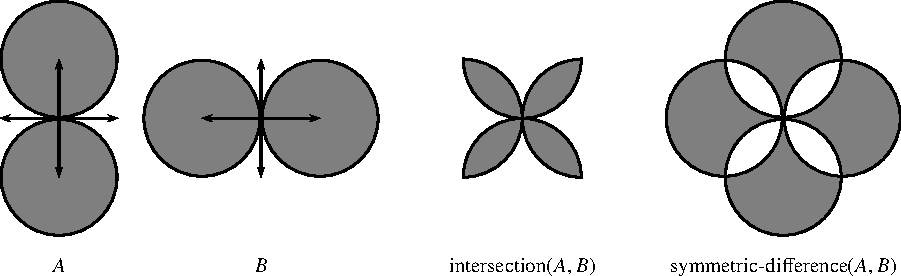
\includegraphics{Boolean_set_operations_2/fig/teaser}
\end{ccTexOnly}
\label{fig:teaser}
\begin{ccHtmlOnly}
  <p><center>
    <img src="./fig/teaser.gif" border=0 alt="Boolean Set-Operations">
  </center>
\end{ccHtmlOnly}
\caption{Examples of Boolean set-operations on general polygons.} 
\end{center}
\end{figure}

This package consists of the implementation of Boolean set-operations
on point sets bounded by $x$-monotone curves\footnote{A continuous
planar curve $C$ is {\em $x$-monotone} if every vertical line intersects it at
most once. We also allow vertical line segments, which are considered
{\em weakly} $x$-monotone.} in 2-dimensional Euclidean space. In particular,
it contains the implementation of {\em regularized} Boolean set-operations,
intersection predicates, and point containment predicates.
Figure~\ref{fig:teaser} shows simple examples of such operations.

A regularized Boolean set-operation $\mbox{op}^*$ can be obtained by
first taking the interior of the resultant point set of an {\em ordinary}
Boolean set-operation $(P\ \mbox{op}\ Q)$ and then by taking the
closure~\cite{cgal:h-sm-04}. That is,
$P\ \mbox{op}^*\ Q = \mbox{closure}(\mbox{interior} (P\ \mbox{op}\ Q))$.
Regularized Boolean set-operations appear in Constructive Solid
Geometry (CSG), because regular sets are closed under regularized
Boolean set-operations, and because regularization eliminates lower
dimensional features, namely isolated vertices and antennas, thus
simplifying and restricting the representation to physically meaningful
solids. Our package provides regularized operations on polygons and
general polygons, where the edges of a general polygon may be
general $x$-monotone curves, rather than being simple line segments.
Ordinary Boolean set-operations, which distinguish between the
interior and the boundary of a polygon, are not implemented within this
package. The \ccc{Nef_2} package supports these operations for (linear)
polygons; see Chapter~\ref{chap:nef_2}. In the rest of this chapter we
use the traditional notation to designate regularized operations; e.g.,
$P \cap Q$ means the regularized intersection of $P$ and $Q$.

A polygon $P$ is said to be {\em simple} (or Jordan) if the
only points of the plane belonging to two polygon edges of $P$ are the
polygon vertices of $P$ --- namely, the polygon edges are pairwise disjoint
in their interior. Such a polygon has a well-defined interior
and exterior and is topologically equivalent to a disk. A polygon in our
context must be simple and its vertices must be ordered in a counterclockwise
direction around the interior of the polygon.
 
\lcTex{%
  \setlength{\widthRight}{1.4cm}
  \setlength{\widthLeft}{\widthLineReal}
  \addtolength{\widthLeft}{-\widthRight}
  \begin{minipage}{\widthLeft}
}
\label{fig:non_strictly_simple_polygon}
\begin{ccHtmlOnly}
  <p><center>
    <img src="./fig/non_strictly_simple.gif" border=0 alt="A non strictly simple polygon" align=right>
  </center>
\end{ccHtmlOnly}
The counterclockwise cyclic sequence of alternating polygon edges and
polygon vertices is referred to as the polygon {\em boundary}.
A polygon whose boundary contains the same vertex twice or more is connected
and simple but not necessarily strictly simple, such as the polygon depicted
on the right.  We extend the notion of a polygon to a point set in $\reals^2$
that has  a topology of a polygon and its boundary edges must map to
$x$-monotone curves, and refer to it as a {\em general polygon}. We sometimes use
the term {\em polygon} instead of general polygon for simplicity hereafter.
\lcTex{%
  \end{minipage}\hspace{\minipageSpace}
  \begin{minipage}{\widthRight}
    \begin{center}
    
\includegraphics{Boolean_set_operations_2/fig/non_strictly_simple}
    \end{center}
%    A non strictly simple polygon.
  \end{minipage}
}

Our package supports the following Boolean set-operations on two point
sets $P$ and $Q$ that are comprized of general polygons:
\begin{description}
\item[Intersection] computes the intersection $R = P \cap Q$.
\item[Join] computes the union $R = P \cup Q$.
\item [Difference] computes the difference $R = P \setminus Q$.
\item [Symmetric Difference] computes the symmetric
  \ccHtmlNoLinksFrom{difference} $P = P \oplus Q = (P \setminus Q) \cup (Q \setminus P)$.
\item[Complement] computes the complement
  \lcTex{$R = \overline{P}$.}
  \lcRawHtml{<i>R = <span style="text-decoration: overline;">P</span>.</i>}
\item [Intersection predicate] tests whether the two sets $P$ and $Q$
  overlap, designating three possible scenarios: (i) the two sets intersect
  on their interior (that is, their regularized intersection is not
  empty $P \cap Q \neq \emptyset$); (ii) the boundaries of two sets intersect
  but their interiors are disjoint; namely they have a finite number
  of common points or even share a boundary curve (still in this case
  $P \cap Q = \emptyset$; and (iii) the two sets are disjoint.
\end{description}
At any case, the set $R$ resulting from a regularized Boolean set-operation
is considered as being a closed point-set.

In the rest of this chapter we review the Boolean set-operations package
in more depth. In Section~\ref{bops_sec:bops_lin} we focus on Boolean 
set-operations on linear polygons, introducing the notion of polygons with 
holes and of a general polygon set. Section~\ref{bops_sec:bops_gen}
introduces general polygons.
We first discuss polygons whose edges are either line segements or circular
arcs and then explain how to construct and use general polygons whose edges
can be arbitrary $x$-monotone curves.

% =================================================
\section{Boolean Set-Operations on Linear Polygons}
\label{bops_sec:bops_lin}
% =================================================

The basic library of \cgal\ includes the \ccc{Polygon_2<Kernel,Container>}
class-template that represents a linear polygon in the plane. The polygon
is represented using a container of \ccc{Kernel::Point_2} objects, namely
its vertices, where its edges are line segments (\ccc{Kenrel::Segment_2}
objects) between adjacent points in the container. By default, the
\ccc{Container} paramters is a vector of \ccc{Kernel::Point_2} objects.

In this section we use the term {\em polygon} to designate a \ccc{Polygon_2}
instance, namely a polygon having linear edges. General polygons are only
discussed in Section~\ref{bops_sec:bops_gen}.

The basic components of our package are the free (global) functions
\ccc{complement()},
\ccc{intersection()}, \ccc{join()},\footnote{As the word \ccc{union} is
a reserved word in {C}{\tt ++}, the function that computes the union of
two polygons is called \ccc{join()}.}, \ccc{difference()},
\ccc{symmetric_difference()} and the predicate \ccc{do_intersect()} that
accept two \ccc{Polygon_2} instances $P$ and $Q$ as their input. We next
explain how these functions should be used throught several examples.

% ~~~~~~~~~~~~~~~~~~~~~~~~~~~~~~~
\subsubsection*{A Simple Example}
% ~~~~~~~~~~~~~~~~~~~~~~~~~~~~~~~

\lcTex{%
  \vspace{-20pt}
  \setlength{\widthRight}{1.4cm}
  \setlength{\widthLeft}{\widthLineReal}
  \addtolength{\widthLeft}{-\widthRight}
  \begin{minipage}{\widthLeft}
}
\label{fig:example}
\begin{ccHtmlOnly}
  <p><center>
    <img src="./fig/triangles.gif" border=0 alt="Two triangles" align=right>
  </center>
\end{ccHtmlOnly}
Testing whether two polygons intersect results with a Boolean value, 
and does not require any additional data beyond the provision of the 
two input polygons. The example listed below tests whether the two
triangles depicted on the right intersect.
\lcTex{%
  \end{minipage}\hspace{\minipageSpace}
  \begin{minipage}{\widthRight}
    \vspace{20pt}
    \begin{center}
    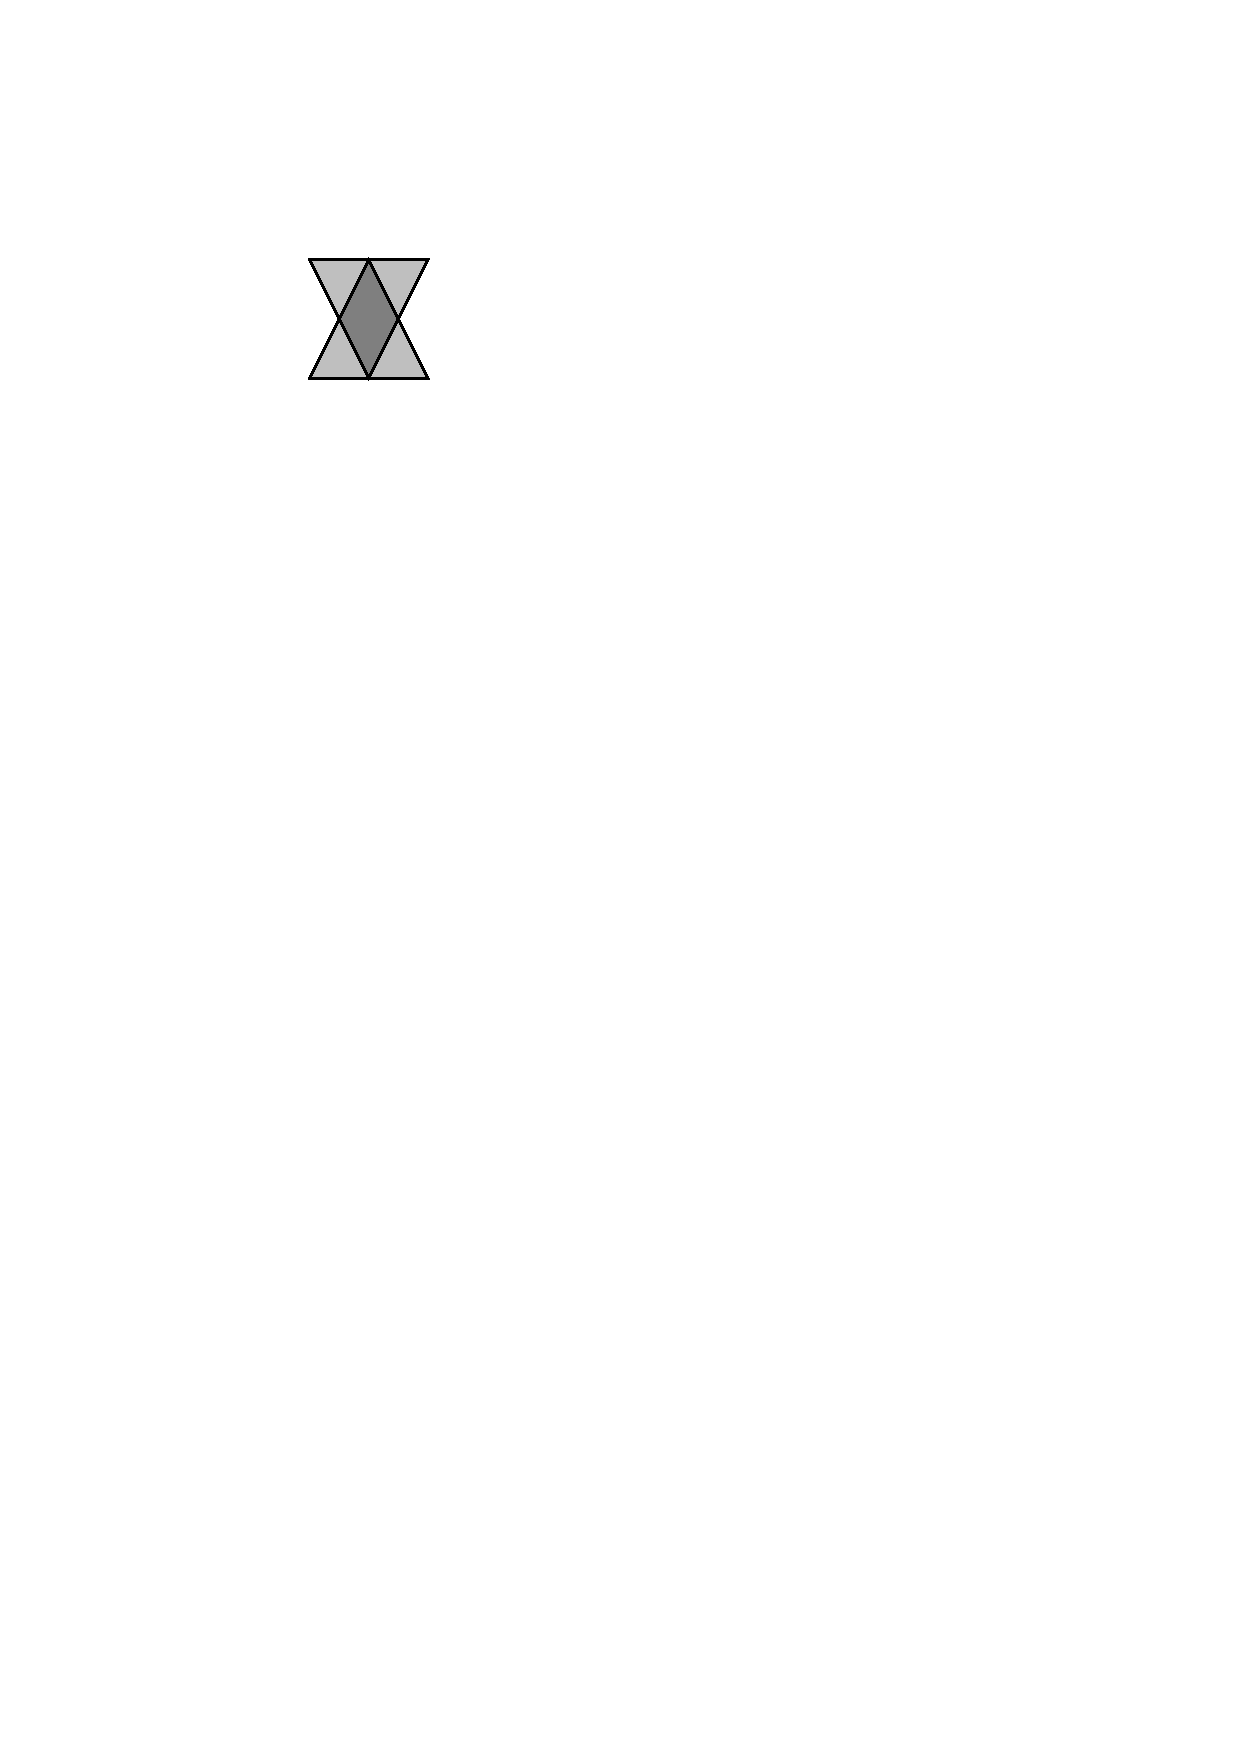
\includegraphics{Boolean_set_operations_2/fig/triangles}
    \end{center}
  \end{minipage}
}

\lcTex{\vspace{-20pt}}
\ccIncludeExampleCode{../examples/Boolean_set_operations_2/ex_do_intersect.C}

% ----------------------------------
\subsection{Polygons with Holes}
\label{bops_ssec:polygons_with_holes}
% ----------------------------------

\begin{figure}[!htp]
\begin{ccTexOnly}
  \begin{center}
  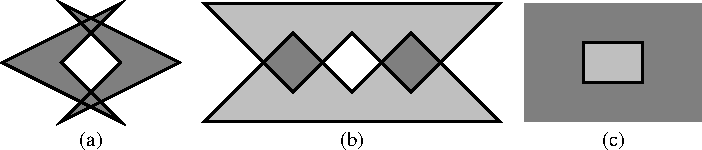
\includegraphics{Boolean_set_operations_2/fig/simple}
  \end{center}
\end{ccTexOnly}
\label{fig:simple}
\begin{ccHtmlOnly}
  <p><center>
    <img src="./fig/simple.gif" border=0 alt="Operations on Strictly
    simple polygons">
  </center>
\end{ccHtmlOnly}
\caption{Operations on strictly simple polygons. (a)~The union of two
polygons, resulting in a point set whose outer boundary is defined by
a simple polygon and contains a polygonal hole in its interior. (b)~The
intersection (darkly shaded) of two polygons (lightly shaded), resulting
in two disjoint polygons. (c)~The complement (darkly shaded) of a strictly
simple polygon (lightly shaded).} 
\end{figure}

In many cases a binary operation that operates on two strictly simple
polygons that have may result in more complicated sets, such as a polygon
that contains holes in its interior (see Figure~\ref{fig:simple}~(a)), 
or a set of disjoint polygons (see Figure~\ref{fig:simple}~(b); a similar
set may result from the union, or the symmetric difference, of two disjoint
polygons). Moreover, the complement of a simple polygon is an unbounded set
that contains a polygons hole; see Figure~\ref{fig:simple}~(c).

It is therefore clear that the free functions cannot output simple polygons.
We therefore introduce the concept \ccc{GeneralPolygonWithHoles_2}. A type
that models this concept represents a set that may be bounded or unbounded.
In case of a bounded set, its {\em outer boundary} is represented as a simple
(but not necessarily strictly simple) polygon whose vertices are oriented in
a counterclockwise order around the interior of the set. In addition, the
set may contain {\em holes}, where each hole is represented as a strictly simple
polygon whose vertices are oriented in a clockwise order around the interior
of the hole. We note that an unbounded polygon having no holes spans the
entire plane. 

Note that vertices of holes may coincide with vertices of the boundary, or may
lie on boundary edges. As the point set represented by a polygon with holes is
considered to be closed, the boundaries of the holes are parts of the set
and are not contained in the holes --- thus, such vertices are considered to
be included in the point set.
\lcTex{%
  \setlength{\widthRight}{1.4cm}
  \setlength{\widthLeft}{\widthLineReal}
  \addtolength{\widthLeft}{-\widthRight}
  \begin{minipage}{\widthLeft}
}
\label{fig:unique}
\begin{ccHtmlOnly}
  <img src="./fig/unique.gif" border=0 alt="Unique" align=right>
\end{ccHtmlOnly}
Consider, for example, the regular set depicted to the right, which is the
result of the union of three small triangles translated appropriately.
(Alternatively, we can reach the same set by taking the
\ccHtmlNoLinksFrom{difference} between a large triangle and a small
upside-down triangle. In general, there are infinitely many ways to arrive at
a particular point set, but we guarantee that the represntation of the
resulting set in unique.) The set is represented as a single polygon having a
triangular outer boundary with a single triangluar hole in its interior ---
and not as three triangles that have no holes at all. As a general rule,
if two point sets areconnected, then they belong to the same polygon with
holes.
\lcTex{%
  \end{minipage}\hspace{\minipageSpace}
  \begin{minipage}{\widthRight}
    \begin{center}
    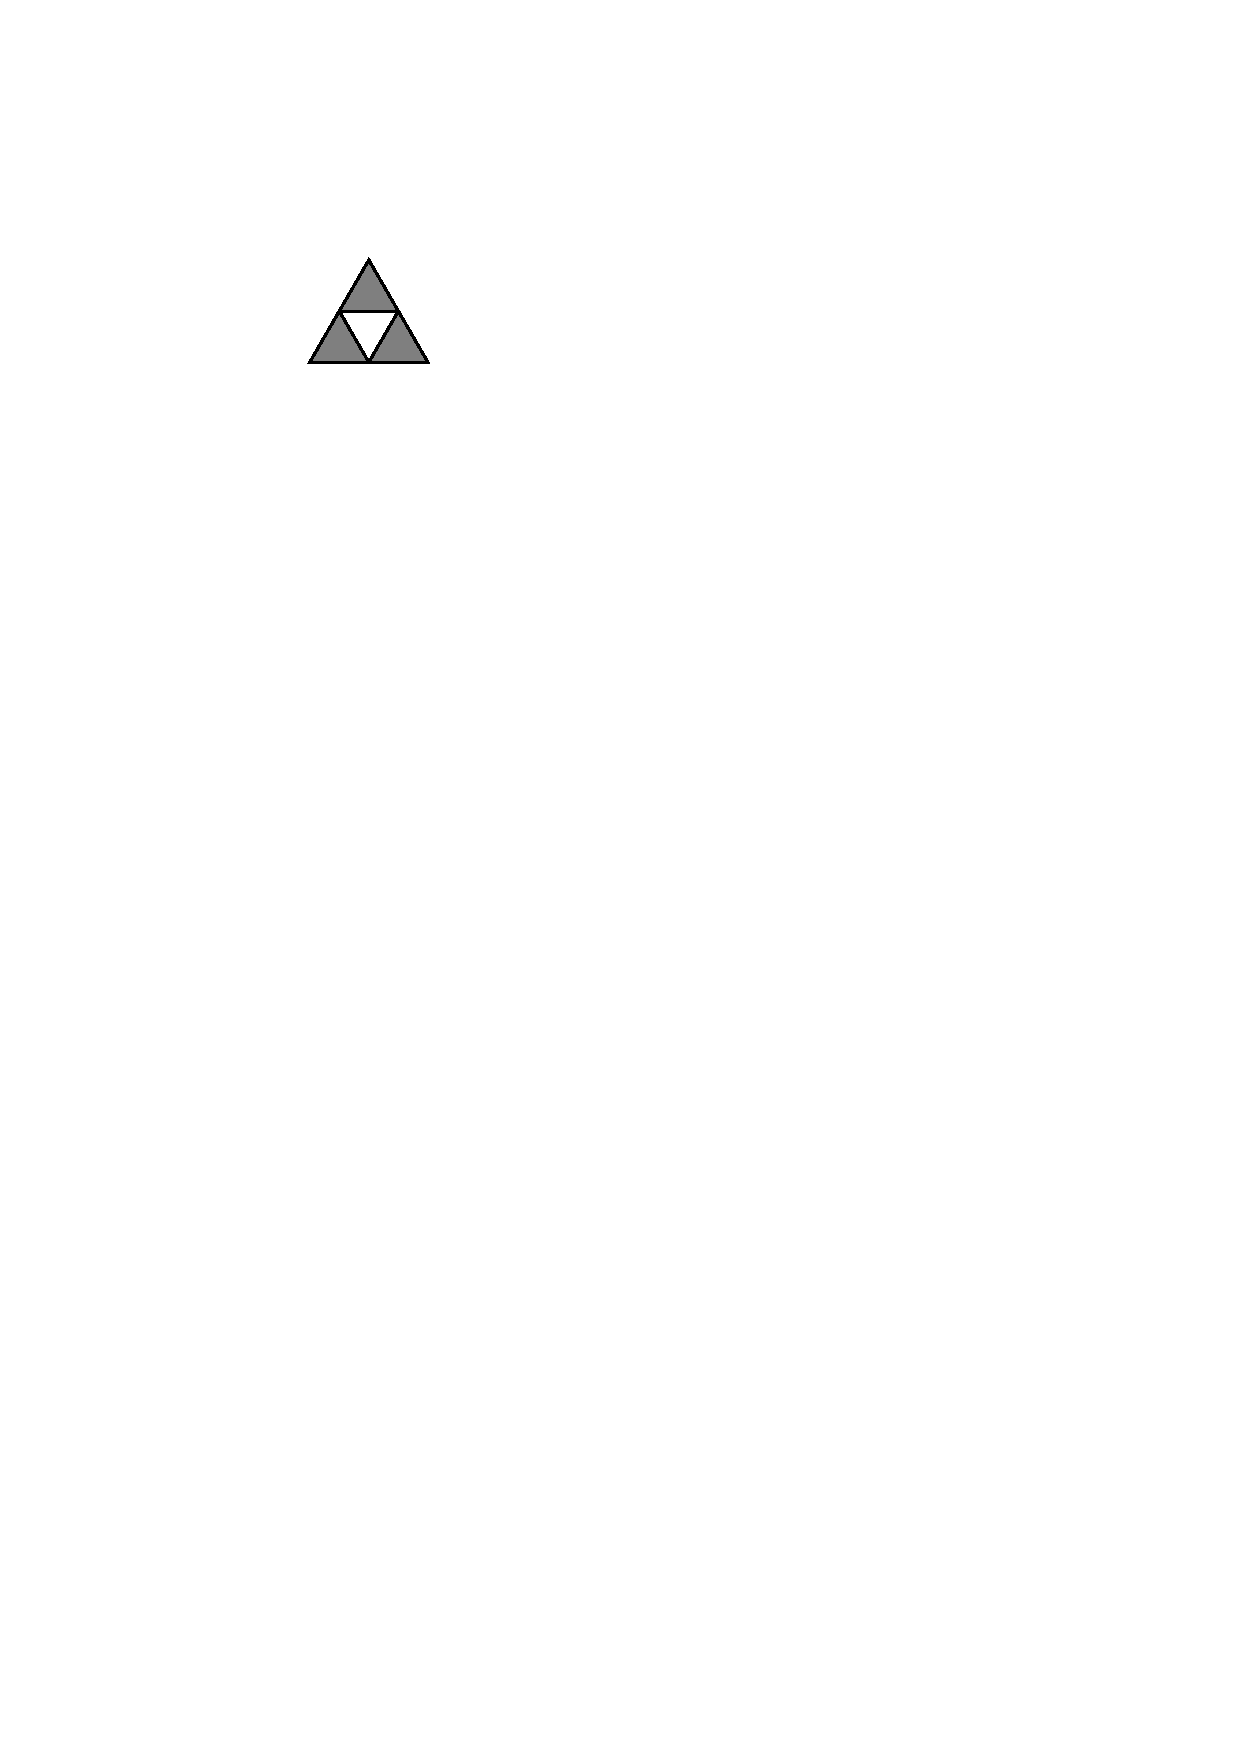
\includegraphics{Boolean_set_operations_2/fig/unique}
    \end{center}
  \end{minipage}
}

The class template \ccc{General_polygon_with_holes_2<Polygon>} represents
polygons with holes as described above, where the outer boundary and the
holes boundaries are realized as \ccc{Polygon} objects. In our context,
the \ccc{Polygon} parameter corresponds to an instantiation of the
\ccc{Polygon_2<Kenrel,Container>} template. Given an instance $P$ of a
\ccc{General_polygon_with_holes_2} class, we can use the predicate 
\ccc{is_bounded()} to check whether $P$ is a bounded set. If it is,
we can obtain the counterclockwise-oriented polygon that represents its
outer boundary by calling the member function \ccc{outer_boundary()}.
It is also possible to traverse the holes of $P$ by invoking
\ccc{holes_begin()} and \ccc{holes_end()}. The two functions return
iterators of the nested type
\ccc{General_polygon_with_holes_2::Hole_const_iterator} that
defined the valid range of $P$'s holes. The value type of this iterator
is \ccc{Polygon_2}.

The simple version of the free functions we have mentioned therefore
accept two \ccc{Polygon_2} instances $P$ and $Q$ as their input, while
their output is given using polygon with holes instances:
\begin{itemize}
\item The complement of a simple polygon $P$ is always an unbounded set
with a single polygonal hole. The function \ccc{complement(P)} therefore
returns a polygon-with-holes instance that represents the complement of $P$.
\item The union of two polygons $P$ and $Q$ is always a single connected
set, unless of course the two input polygons are completely disjoint. In
the latter case $P \cup Q$ trivially consists of the two input polygons.
The free function \ccc{join(P, Q, R)} therefore returns a Boolean value
indicating whether $P \cap Q \neq \emptyset$. If the two polygons are not
disjoint, it assignes the a polygon with holes $R$ instance (which it
accepts by reference) by the union of the regularized union operation
$P \cup Q$.
\item The other three functions, namely \ccc{intersection(P, Q, oi)}, 
\ccc{difference(P, Q, oi)} and \ccc{symmetric_difference(P, Q, oi)}, all
have a similar interface. As the result of these operation may consist of
several disconnected components, they all accept an output iterator \ccc{oi},
whose value type is \ccc{General_polygon_with_holes_2}, and write the
output polygons to it.
\end{itemize}

% ~~~~~~~~~~~~~~~~~~~~~~~~~~~~~~~~~~~~~~~~~~~~~~~~~~~~~~~~~~~~~~~~~~
\subsubsection{Example --- Joining an Intersecting Simple Polygons}
\label{bops_sssec:ex_simple_bops}
% ~~~~~~~~~~~~~~~~~~~~~~~~~~~~~~~~~~~~~~~~~~~~~~~~~~~~~~~~~~~~~~~~~~

The following example demonstartes the usage of the free functions
\ccc{join()} and \ccc{intersect()} for computing the union and the
intersection of the two simple polygons depicted in
Figure~\ref{fig:simple}~(b).


Suppose that you need to compute the union of two general polygons. If the
two polygons are disjoint, the result is a pair that consists of the two 
original polygons. Otherwise, it is a single general polygon perhaps with 
holes. This observation is used to simplify the interface of the free
functions that compute the union of two general polygons. These functions
return \ccc{false} iff the polygons are disjoint, and \ccc{true} otherwise,
in which case the resulting general polygon is placed in a third argument 
passed by reference.

\ccIncludeExampleCode{../examples/Boolean_set_operations_2/ex_simple_join_intersect.C}

% ~~~~~~~~~~~~~~~~~~~~~~~~~~~~~~~~~~~~~~~~~~~~~~~
\subsubsection{Operations on Polygons with Holes}
\label{bops_sssec:pwh_bops}
% ~~~~~~~~~~~~~~~~~~~~~~~~~~~~~~~~~~~~~~~~~~~~~~~

Having introduced polygons with holes and explained how the free functions
output such objects, it is only natural to perform operations on sets that
are represented as polygon with holes, rather than simple polygons.
Indeed, the Boolean set-operations package provides overriden free functions
\ccc{complement()}, \ccc{intersection()}, \ccc{join()}, \ccc{difference()},
\ccc{symmetric_difference()} and \ccc{do_intersect()} that accept
\ccc{General_polygon_with_holes_2} instances as their input. The prototypes of
most functions is the same as these of their simpler counterparts that operate
on simple polygon. The only exception is \ccc{complement(P, oi)}, which
outputs a range of polygons with holes that represent the complement of the
polygon with holes $P$.

In the following example we demonstrate how to compute the symmetric
difference between two sets that contain holes. Each set is a rectangle that
contains a rectangular hole in its interior, such that the symmetric
difference between the two sets is a single polygon that consists of five
holes:

\ccIncludeExampleCode{../examples/Boolean_set_operations_2/ex_symmetric_difference.C}

% ------------------------------------
\subsection{Operating on Polygon Sets}
\label{bops_sec:main_component}
% ------------------------------------

We have argued that the result of a regularized operations on two polygons
(or polygons with holes) $P$ and $Q$ is typically a collection of several
disconnected polygons with holes. It is only natural to represent such a
collection in terms of a class, making it possible to operate on the set
resulting from computing, for example, $P \setminus Q$.

The central component in the Boolean set-operations package is the
\ccc{General_polygon_set_2} class-template. An instance of this class
represents a point set formed by the collection of several disconnected
polygons with holes. It employs the \ccc{Arrangement_2} class to represent
this point set in the plane as a planar arrangement; see
Chapter~\ref{chapterArrangement_2}. 

An instance $S$ of a \ccc{General_polygon_set_2} class usually represents
the result of a sequence of operations that were applied on some input
polygons. The representation of $S$ is unique, regardless of the particular
sequence of operations that were applied in order to arrive at it.

In addition, a polygon-set instance can be constructed from a single polygon
instance or from a polygon-with-holes instance. Once constructed, it is
possible to add new polygons (or polygons with holes)
into the set using the \ccc{insert()} method, as long as the inserted
polygons are disjoint from the existing polygons in the set. 
The \ccc{General_polygon_set_2} class also provide access functions for
the polygons with holes it contains, and a few queries. The most improtant
query is $\ccc{S.oriented_side(q)}$ which determined whether the query point
$q$ lies in the interior of the set $S$, on the boundary of the set, or
whether it is not in the set.

The \ccc{General_polygon_set_2} class defines the predicate
\ccc{do_intersect()} and the methods \ccc{complement()}, \ccc{intersection()},
\ccc{join()}, \ccc{difference()} and \ccc{symmetric_difference()} as member
functions. The operands to these functions may be simple polygons 
(\ccc{Polygon_2} inatnces), polygons with holes 
(\ccc{General_polygon_with_holes_2} instances), or polygon sets
(\ccc{General_polygon_set_2} instances). Thus, each of the function mentioned
above is actually realized by a set overriding member functions.

Member functions of the \ccc{General_polygon_set_2} that perform
Boolean set-operations come in two flavors: for example, \ccc{S.join(P, Q)}
computes the union of $P$ and $Q$ and assigned the reuslt to $S$, while
\ccc{S.join(P)} preformes the operation $S \longleftarrow S \cup P$.
Similarly, \ccc{S.complement(P)} sets $S$ to be the complement of $P$ while
$S.complement()$ simply negates the set $S$.

% ~~~~~~~~~~~~~~~~~~~~~~~~~~~~~~~~~~~~~~~~~~
\subsubsection{A Sequence of Set Operations}
\label{bops_sssec:sequence}
% ~~~~~~~~~~~~~~~~~~~~~~~~~~~~~~~~~~~~~~~~~~

The free functions we reviewed in Section~\ref{bops_ssec:polygons_with_holes}
serve as a wrapper for the polygon-set class and are only provided for
convinience. A typical such function constructs a pair of 
\ccc{General_polygon_set_2} instances, invokes the 
appropriate method to apply the desired Boolean operation, and transforms
the resulting polygon set to the required output format.
It should therefore be clear that when several operations are 
performed in a sequence, it is much more efficient to use the member 
functions of the \ccc{General_polygon_set_2} type directly, as the 
extraction of the polygons from the internal representation for some 
operation, and the reconstruction of the internal representation for 
the succeeding operation could be time consuming.

\lcTex{%
  \setlength{\widthRight}{2.3cm}
  \setlength{\widthLeft}{\widthLineReal}
  \addtolength{\widthLeft}{-\widthRight}
  \begin{minipage}{\widthLeft}
}
\label{fig:sequence}
\begin{ccHtmlOnly}
  <p><center>
    <img src="./fig/sequence.gif" border=0 alt="A sequence of operation" align=right>
  </center>
\end{ccHtmlOnly}
The next example performs a sequence of three Boolean set-operations.
First, it computes the union of two simple polygons depicted in
Figure~\ref{fig:simple}~(a). It then computes the complement of the result
of the union operation. Finally, it computes the intersection of the result
of the complement operation with a rectangle, confining the final result to 
the area of the rectangle.
\lcTex{%
  \end{minipage}\hspace{\minipageSpace}
  \begin{minipage}{\widthRight}
    \begin{center}
    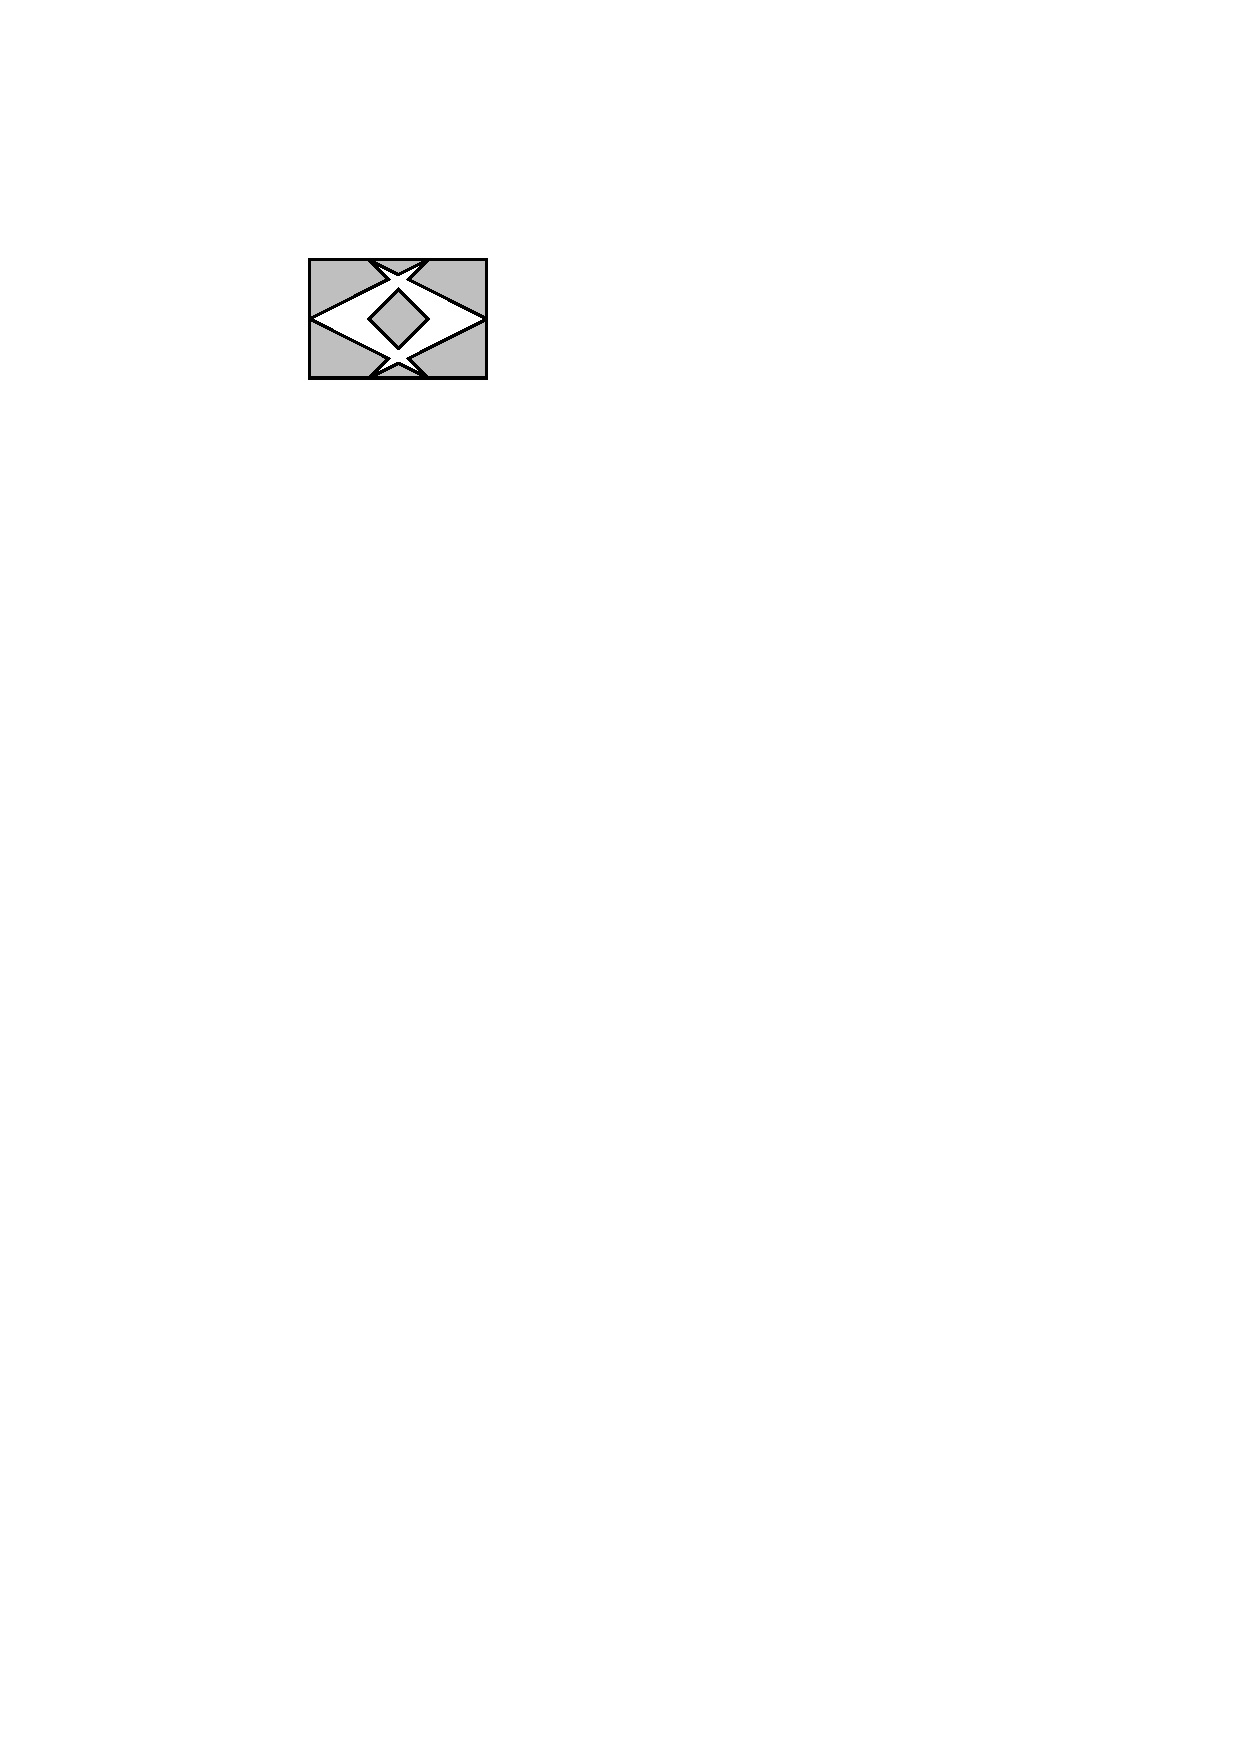
\includegraphics{Boolean_set_operations_2/fig/sequence}
    \end{center}
  \end{minipage}
  \vspace{2pt}
}

\ccIncludeExampleCode{../examples/Boolean_set_operations_2/ex_sequence.C}

% ~~~~~~~~~~~~~~~~~~~~~~~~~~~~~~~~~~~~~~~~~~~~~~~~~
\subsubsection{Inserting Non Intersecting Polygons}
\label{bops_ssec:insert_ni}
% ~~~~~~~~~~~~~~~~~~~~~~~~~~~~~~~~~~~~~~~~~~~~~~~~~

As we have mentioned before, in order to compute the union of a polygon $P$
($P$ may be a simple polygon or a polygon-with-holes instance)
with a polygon set $S$, and store the result in $S$, we should use the
following lines of code:
\begin{alltt}
  Polygon_set_2  setP (P);
  S.join (setP);
\end{alltt}
As a matter of fact, it is even easier to directly apply union operation
that accepts a single polygon:
\begin{alltt}
  S.join (P);
\end{alltt}

If, however, it is known in advance that $P$ is disjoint from all polygons
currently stored in $S$, it is more efficient to simply insert it into the
\begin{alltt}
  S.insert (P);
\end{alltt}
As \ccc{insert()} assumes that $P \cap S = \emptyset$, it does try to
compute intersections between the boundaries of $P$ and of $S$. This fact
significantly speeds the insertion process in comparison with the insertion
of a non-disjoint polygon that intersects $S$.

The \ccc{join()} function is also overloaded, so it can also accept a range
of polygons. When a range of polygons are inserted into a polygon set $S$,
all the general polygons in the range and the general polygons represented
by $S$ must be pairwise disjoint in their interiors.

% -------------------------------------------
\subsection{Performing Aggregated Operations}
\label{bops_ssec:agg_ops}
% -------------------------------------------

Assume that we are given a set of polygons $P_1, \ldots P_m$ and wish
to compute their union. This can be done of course incrementally, by
computing at each step the union of $S_{k-1} = \bigcup_{i=1}^{k-1}{P_i}$
with $P_{k}$ and obtaining $S_k$. Namely, if our polygon set is given
as a pair of iterator \ccc{[begin, end)}, we use the following code
fragment:
\begin{alltt}
  InputIterator   iter = begin;
  Polygon_set_2   S (*iter);

  ++iter;
  while (iter != end) 
  \{
    S.join (*iter);
    ++iter;
  \}
\end{alltt}  
Alternaitvely, the same result can be obtained using a divide-and-conquer
approach, by recursively computing $S_1$ and $S_2$, each represents the
union of half of the polygons, then computing $S_1 \cup S_2$.

However, this union operation can be done more efficiently for sparse polygons,
having a relatively small number of intersections, by simultaneously computing
the union of all polygons. This is done by constructing a planar arrangement
of all input polygons, utilizing the sweep-line algorithm, then extracting
the result from this arrangement. Similarly, it is possible to aggregately
compute the union $\bigcap_{i=1}^{m}{P_i}$ of a set of input polygons.

Our package provides the free overloaded functions \ccc{join()} and
\ccc{intersect()} that aggregately compute the union and the intersection
of a range of input polygons. There is no restriction on the polygons in the
range --- naturally, they may intersect each other.
The package provides the overloaded free function 
\ccc{do_intersect(begin, end)} that determines whether the polygons in the
range defined by the two input iterators \ccc{[begin, end)} intersect.

The class \ccc{General_polygon_set_2} also provides equivalent member
functions that aggragately operate on a range of input polygons or
polygons with holes. When such a member function is called, the general 
polygons represented by the current object are considered operands as 
well. Thus, we can easily compute the union of our polygon range by
writing:
\begin{alltt}
  Polygon_set_2   S;
  S.join (begin, end);
\end{alltt} 


% ==================================================
\section{Boolean Set-Operations on General Polygons}
\label{bops_sec:bops_gen}
% ==================================================

\lcTex{%
  \setlength{\widthRight}{1.4cm}
  \setlength{\widthLeft}{\widthLineReal}
  \addtolength{\widthLeft}{-\widthRight}
  \begin{minipage}{\widthLeft}
}
\label{fig:general_polygon}
\begin{ccHtmlOnly}
  <p><center>
    <img src="./fig/general_polygon.gif" border=0 alt="A general polygon" align=right>
  </center>
\end{ccHtmlOnly}
So far we have dealt with ordinary polygons, namely closed point set bounded
by a piecewise linear curves. The Boolean set-operations package allows
a more general geometric mapping of the polygon edges. The operations provided
by the package operate on point sets bounded by $x$-monotone segments of
general curves (e.g., conic arcs and segments of polynomial functions).
For example, the point set depicted on the right is general polygon bounded
by two $x$-monotone circular arcs.
\lcTex{%
  \end{minipage}\hspace{\minipageSpace}
  \begin{minipage}{\widthRight}
    \begin{center}
    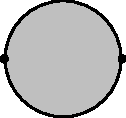
\includegraphics{Boolean_set_operations_2/fig/general_polygon}
    \end{center}
%    A general polygon.
  \end{minipage}
  \vspace{2pt}
}\\

The central class \ccc{General_polygon_set_2} that offers
methods that implement these operations is parameterized by a {\em traits}
class that defines the type points used to represent polygon vertices and
the of $x$-monotone curves that represent the polygon edges. The traits
class also the primitive geometric operations on objects of these types.

% ------------------------------------
\subsection{The Traits-Class Concepts}
\label{bops_ssec:traits_concepts}
% ------------------------------------

The traits class must be a model of the concept
\ccc{GeneralPolygonSetTraits_2}, and is tailored to handle a specific 
family of curves. The concept \ccc{GeneralPolygonSetTraits_2} refines the 
concept \ccc{ArrangementDirectionalXMonotoneTraits} specified next.

The concept \ccc{ArrangementDirectionalXMonotoneTraits} refines the 
concept \ccc{ArrangementXMonotoneTraits_2} (see 
Section~\ref{arr_sssec:insert_x_mon} in the 2D Arrangements chapter).
Thus, a model of this concept must define the type \ccc{X_monotone_curve_2}, 
which represents an $x$-monotone curve, and the type \ccc{Point_2} 
which represents a planar point that may correspond to an endpoint of an
$x$-monotone curve or to an intersection point between two curves.
It must also provide various geometric predicates and operations 
on these types listed by the base concept, such as determining whether
a point lies above or below an $x$-monotone curve, computing the intersections
between two curves, etc. Note that the base concept does not assume that 
$x$-monotone curves are directed: an $x$-monotone curve is not required
to have a designated {\em source} and {\em target}, it is only required to
determine the left (lexicographically smaller) and the right
(lexicographically larger) endpoints of a given curve.

The \ccc{ArrangementDirectionalXMonotoneTraits} concept treats its
$x$-monotone curves as directed objects. It thus requires two additional
operations on $x$-monotone curves:
\begin{itemize}
\item Given an $x$-monotone curve, compare its source and target points
lexicographically.
\item Given an $x$-monotone curve, construct its opposite curve (namely,
swap its source and target points).
\end{itemize}

The traits classes \ccc{Arr_segment_traits_2}, 
\ccc{Arr_non_caching_segment_traits}, \ccc{Arr_circle_segment_traits_2},
\ccc{Arr_conic_traits_2} and \ccc{Arr_rational_arc_traits_2}, which are 
bundeled in the \ccc{Arrangement_2} package and distributed with \cgal,
are all models of the refined concept 
\ccc{ArrangementDirectionalXMonotoneTraits}.\footnote{The
\ccc{Arr_polyline_traits_2} class is {\em not} a model of the, 
\ccc{ArrangementDirectionalXMonotoneTraits} concept, as the
$x$-monotone curve it defines is always directed from left to right. Thus, an
opposite curve cannot be constructed. However, it is not very useful to
construct a polygon whose edges are polylines, as an ordinary polygon
with linear edges can represent the same entity.}

Just as with the case of computations using models of the 
\ccc{ArrangementXMonotoneTraits_2} concept, operations are robust only
when exact arithmetic is used. When inexact arithmetic is used,
(nearly) degenerate configurations may result in abnormal termination
of the program or even incorrect results.

% ---------------------------------------------------------------
\subsection{The Traits Polygons}
\label{bso_ssec:traits_polygons}
% ---------------------------------------------------------------
\lcTex{%
  \setlength{\widthRight}{1.4cm}
  \setlength{\widthLeft}{\widthLineReal}
  \addtolength{\widthLeft}{-\widthRight}
  \begin{minipage}{\widthLeft}
}
\label{fig:general_polygon_with_holes}
\begin{ccHtmlOnly}
  <p><center>
    <img src="./fig/general_polygon_with_holes.gif" border=0 alt="A general polygon with holes" align=right>
  </center>
\end{ccHtmlOnly}
Every model of the traits-class concept must also define the types
\ccc{Polygon_2} and \ccc{Polygon_with_holes_2}, and it must provide
sufficient operations on objects of these types to enable the Boolean 
set-operations.  The type \ccc{Polygon_2} represents a simple point-set 
in the plane, whose boundary curves are $x$-monotone. There are no 
requirements on this type besides being default and copy constructible and
assignable. In other words, the type \ccc{Polygon_2} does not necessari-
\lcTex{%
  \end{minipage}\hspace{\minipageSpace}
  \begin{minipage}{\widthRight}
    \begin{center}
    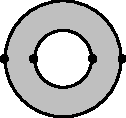
\includegraphics{Boolean_set_operations_2/fig/general_polygon_with_holes}
    \end{center}
%    A general polygon with holes.
  \end{minipage}
  \vspace{1pt}
}\\
ly provide methods to access the curves of the polygon boundary, nor 
does it necessarily provide a constructor from a range of curves. Instead, 
the traits concept requires these operations. The type 
\ccc{Polygon_with_holes_2} corresponds to the concept 
\ccc{GeneralPolygonWithHoles_2}. Recall, that this concept 
requires access to the outer boundary, which is of type \ccc{Polygon_2}, 
and to the holes, where each hole is also of type \ccc{Polygon_2}.
% The \ccc{Triangle_2} and \ccc{Iso_rectangle_2} classes for example,
% which represent a triangle and a parallel-axis rectangle in
% $\mathrm{E}^2$ are special cases of convex general polygon. The a-priori
% knowledge of whether the input polygons are convex may sometimes expedite
% the operation or simplify the representation of the result. For example,
% the intersection of two convex polygons is either an empty polygon or a
% convex polygon.

% ---------------------------------------------------------------
\subsection{Types of Traits}
\label{bso_ssec:traits_types}
% ---------------------------------------------------------------
\lcTex{%
  \setlength{\widthRight}{2.4cm}
  \setlength{\widthLeft}{\widthLineReal}
  \addtolength{\widthLeft}{-\widthRight}
  \begin{minipage}{\widthLeft}
}
\label{fig:circle_recs}
\begin{ccHtmlOnly}
  <p><center>
    <img src="./fig/circles_rects.gif" border=0 alt="Union of circles
    and rectangles" align=right>
  </center>
\end{ccHtmlOnly}
Two traits classes are distributed with \cgal, namely 
\ccc{Gps_segment_traits_2} and \ccc{Gps_circle_segment_traits_2}. 
The former handles linear segments, and uses the \ccc{Polygon_2} type,
which is defined in the Polygons and Polygon Operations package of 
\cgal; see Chapter~\ref{Polygon}. The latter handles circular arcs
and linear segments concurrently. It is parameterized by a rational 
kernel, which makes it extremely efficient. The details are provided in the 
reference manual. The following example uses this traits class to compute
the union of four rectangles and four circles incrementally resulting with 
a single polygon with a single hole, as depicted on the right. Note that as
the four circles
\lcTex{%
  \end{minipage}\hspace{\minipageSpace}
  \begin{minipage}{\widthRight}
    \begin{center}
    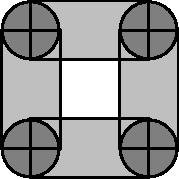
\includegraphics{Boolean_set_operations_2/fig/circles_rects}
    \end{center}
%    A general polygon with holes.
  \end{minipage}
  \vspace{2pt}
}\\
are disjoint, their union is computed with the \ccc{insert} method, 
while the union of the rectangles is computed with the \ccc{join} operator.

\ccIncludeExampleCode{../examples/Boolean_set_operations_2/ex_circle_segment.C}

% ===============================================================
\subsection{General Polygon Set Traits Adaptor}
\label{bso_ssec:general_polygon_concept}
% ===============================================================
The concept \ccc{GeneralPolygon_2} and its generic model 
\ccc{General_polygon_2<ArrDirectionalXMonotoneTraits>} facilitate the 
production of general-polygon set traits classes. A model of the concept 
\ccc{GeneralPolygon_2} represents a simple point-set in the plane bounded 
by $x$-monotone curves. As opposed to the plain \ccc{Traits::Polygon_2} type 
defined by any traits class, it must define the type 
\ccc{X_monotone_curve_2}, which represents an $x$-monotone curve of the 
point-set boundary. It must provide a constructor from a range of such 
curves, and a pair of methods, namely \ccc{curves_begin()} and 
\ccc{curves_end()}, that can be used to iterate over the point-set boundary 
curves.
 
The class-template \ccc{General_polygon_2<ArrDirectionalXMonotoneTraits>}
models the concept \ccc{GeneralPolygon_2}. Its template parameter must be
instantiated with a model of the concept
\ccc{ArrangementDirectionalXMonotoneTraits_2} from which it obtains the 
\ccc{X_monotone_curve_2} type, and it uses the necessary 
operations on this type provided by such a model to maintain a container 
of directed curves of type \ccc{X_monotone_curve_2}, which represents the 
boundary of the general polygon.

The class-template 
\ccc{Gps_traits_2<ArrDirectionalXMonotoneTraits,GeneralPolygon>}
models the concept \ccc{GeneralPolygonSetTraits_2}. Its implementation is 
rather simple, as it is derived from the instantiated template-parameter 
\ccc{ArrXMonotoneTraits} inheriting its necessary types and methods, 
and it exploits the methods provided by the instantiated parameter 
\ccc{GeneralPolygon} --- a model of the concept \ccc{GeneralPolygon_2}.
By default, the \ccc{GeneralPolygon} parameter is defined as
\ccc{General_polygon_2<ArrangementDirectionalXMonotoneTraits_2>}

The code excerpt listed below defines a general-polygon set type that
can be used to perform Boolean set-operations on point sets bounded by
linear segments used by the \ccc{Arrangement_2} class by default. A
model of the \ccc{GeneralPolygon_2} concept that represents a
(linear) polygon bounded by curves of type \ccc{Arr_segment_2} is
generated. The later is obtained from the instantiated parameter
\ccc{Arr_segment_traits_2}, which defines \ccc{Arr_segment_2} to be
its exposed type \ccc{X_monotone_curve_2}.
\begin{alltt}
typedef CGAL::Gmpq                                      Number_type;
typedef CGAL::Cartesian<Number_type>                    Kernel;
typedef CGAL::Arr_segment_traits_2<Kernel>              Arr_traits;
typedef CGAL::General_polygon_2<Arr_traits>             General_polygon;
typedef CGAL::Gps_traits_2<Arr_traits,General_polygon>  Traits;
typedef CGAL::General_polygon_set_2<Traits>             General_polygon_set;
\end{alltt}

\lcTex{%
  \setlength{\widthRight}{5.4cm}
  \setlength{\widthLeft}{\widthLineReal}
  \addtolength{\widthLeft}{-\widthRight}
  \begin{minipage}{\widthLeft}
}
\label{fig:conics}
\begin{ccHtmlOnly}
  <p><center>
    <img src="./fig/conic_arcs.gif" border=0 alt="Conic arcs" align=right>
  </center>
\end{ccHtmlOnly}
Swapping the linear arrangement-traits \ccc{Arr_segment_traits_2}
above with a traits class that handle conic arcs, such as
\ccc{Arr_conic_traits_2}, results with the definition of a
general-polygon set type that can be used to perform Boolean 
set-operations on point sets bounded by conic arcs of type
\ccc{Arr_conic_2}. The next example computes the intersection of the
two general polygons depicted on the right. One is an ellipse
given by $x^2 + 9y^2 - 9 = 0$, and the other is bounded by the two
parabolic arcs whose underlying parabola are given by 
$x^2 + 2y - 4 = 0$, and $x^2 - 2y - 4 = 0$. The code in the example adapts
the traits model that handles conics included with the \ccc{Arrangement_2}
package.
\lcTex{%
  \end{minipage}\hspace{\minipageSpace}
  \begin{minipage}{\widthRight}
    \begin{center}
    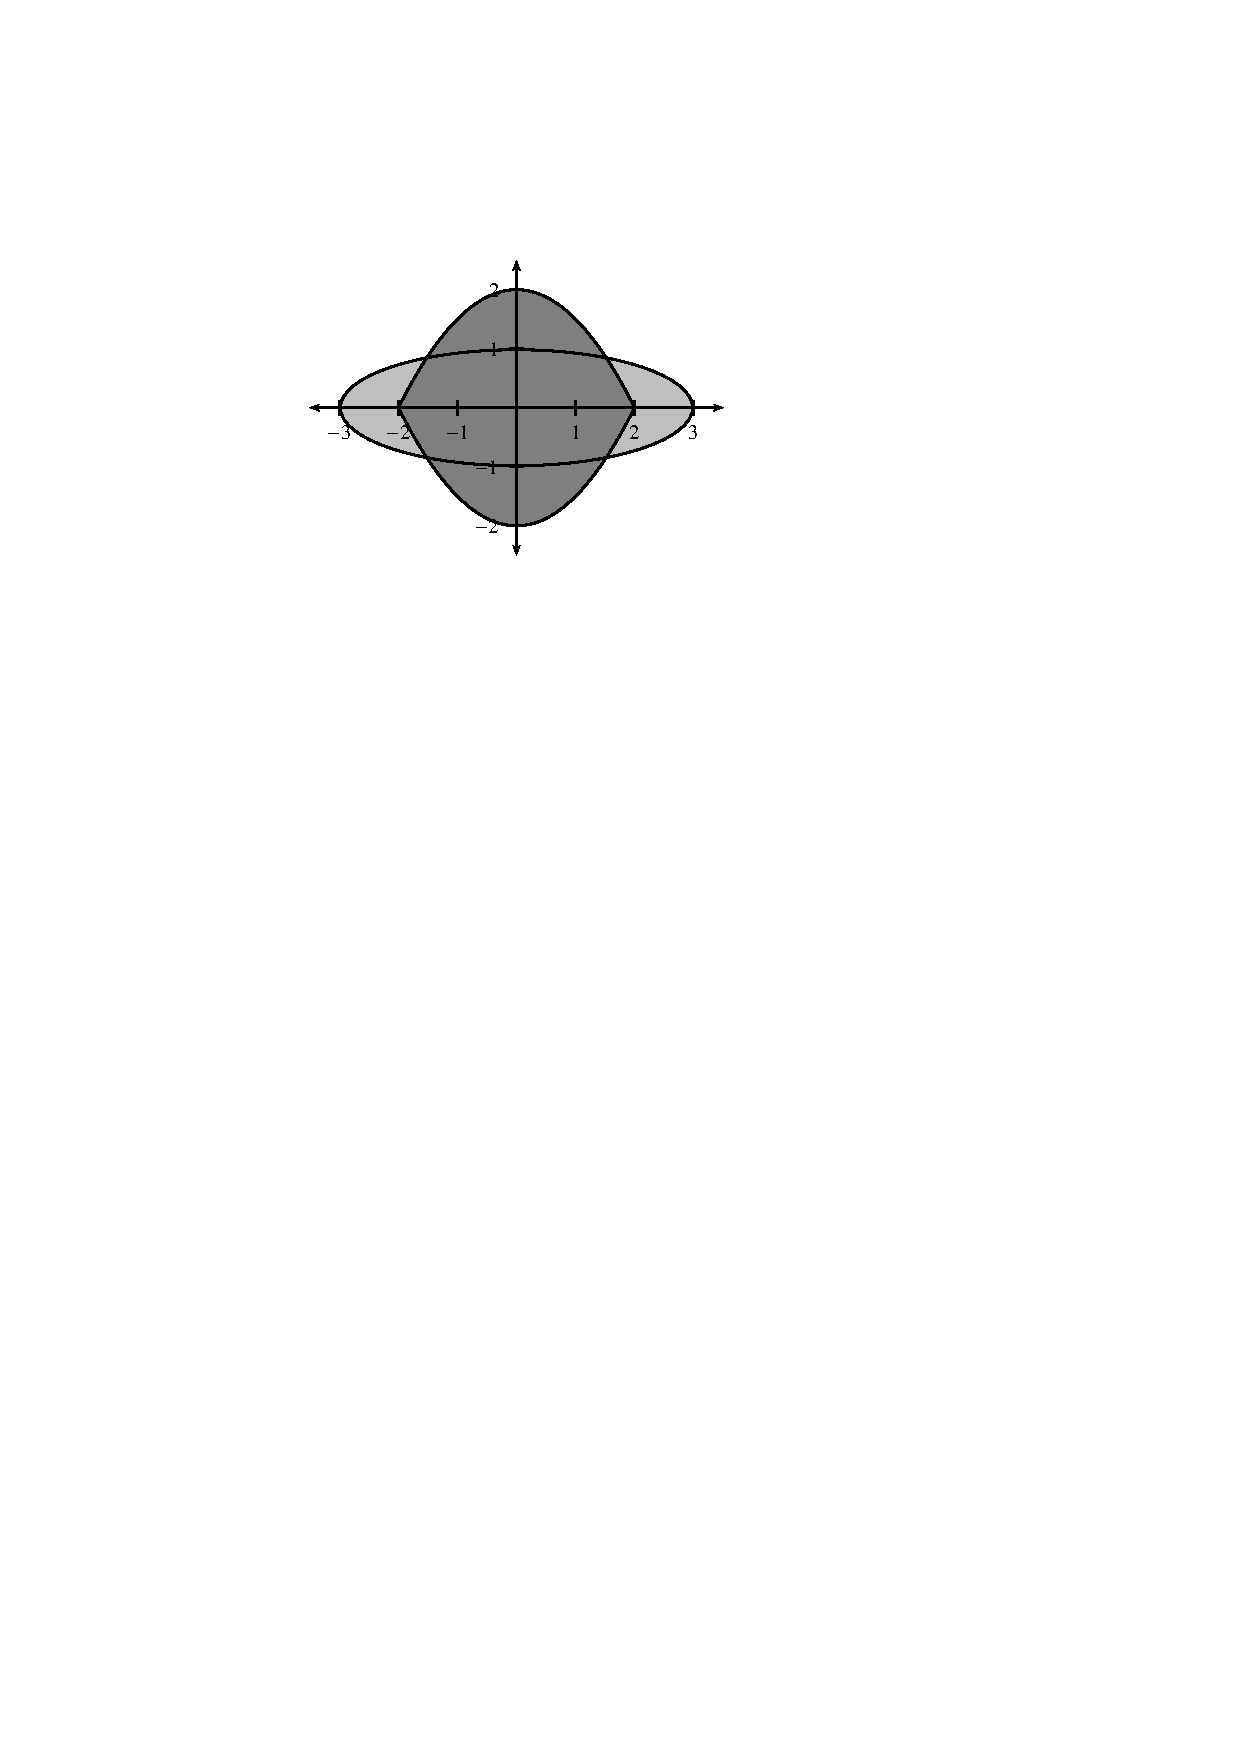
\includegraphics{Boolean_set_operations_2/fig/conic_arcs}
% Conic arcs.
    \end{center}
  \end{minipage}
}

\ccIncludeExampleCode{../examples/Boolean_set_operations_2/ex_traits_adaptor.C}


% ------------------------------------------
\subsection{Example - Aggregated Operations}
\label{bops_ssec:aggregated_gen_ops}
% ------------------------------------------

\lcTex{%
  \setlength{\widthRight}{3.4cm}
  \setlength{\widthLeft}{\widthLineReal}
  \addtolength{\widthLeft}{-\widthRight}
  \begin{minipage}{\widthLeft}
}
\label{fig:disks}
\begin{ccHtmlOnly}
  <p><center>
    <img src="./fig/disks.gif" border=0 alt="Union of disks" align=right>
  </center>
\end{ccHtmlOnly}

\lcTex{%
  \end{minipage}\hspace{\minipageSpace}
  \begin{minipage}{\widthRight}
    \begin{center}
    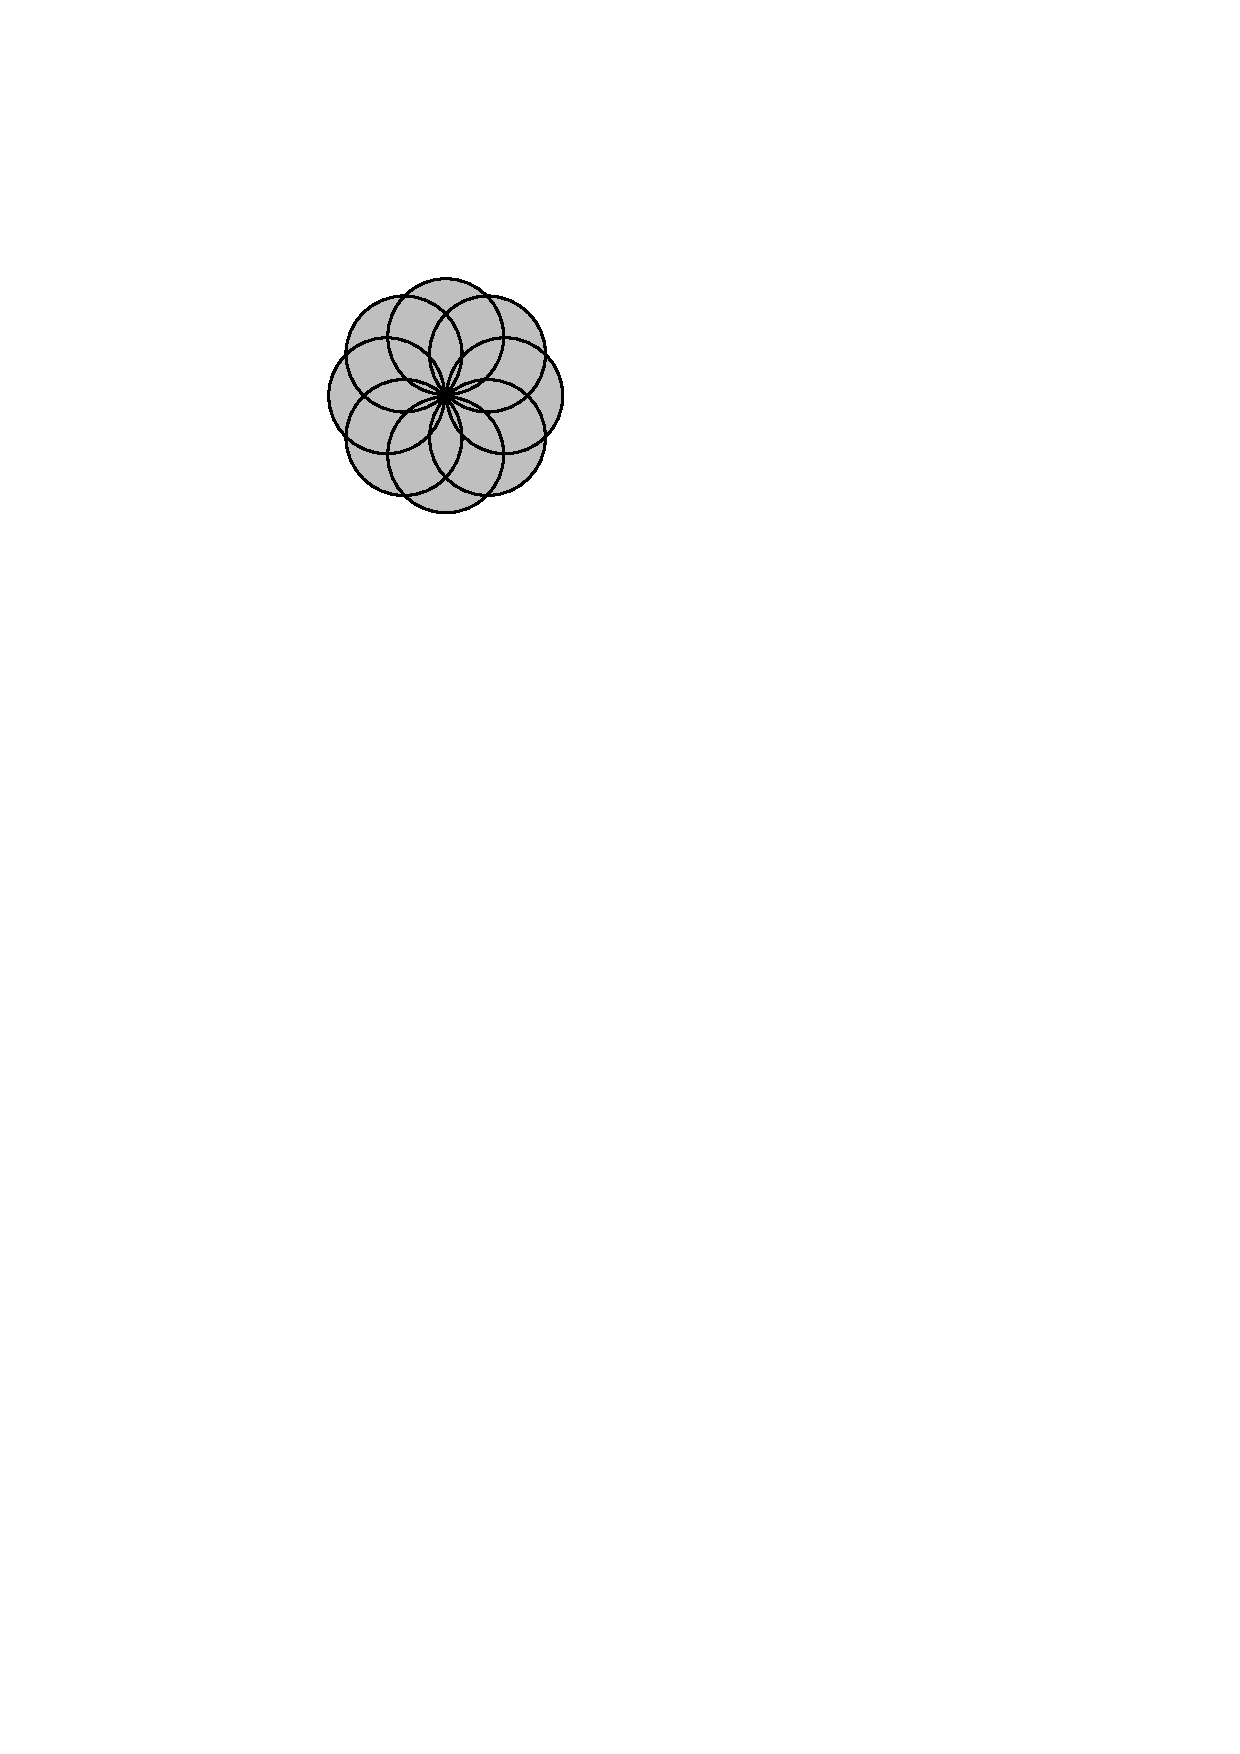
\includegraphics{Boolean_set_operations_2/fig/disks}
    \end{center}
%    Union of disks.
  \end{minipage}
\vspace{2pt}
}\\


\ccIncludeExampleCode{../examples/Boolean_set_operations_2/ex_set_union.C}
